\documentclass[xcolor=dvipsnames]{beamer}
\usepackage[utf8]{inputenc}
\usepackage{xcolor}
\usepackage{graphicx}
\usepackage{MnSymbol}
\usepackage{stmaryrd}
\usepackage{colortbl}
\usepackage{caption}
\usepackage{comment}
\usepackage[utf8]{inputenc}
\usepackage{pdfpages}
\usepackage{listings}
\usepackage{color}
\usepackage{booktabs}
\usepackage{soul}
\usepackage[normalem]{ulem}


\usepackage{tcolorbox}
\usepackage{lipsum}


%%%%%%%%%%%%%%%%%%%%%%%%%%%%%%%%%%%%%%%%%%%%%%%%%

\usepackage{pgf}
\usepackage{etex}
\usepackage{tikz,pgfplots}


\usetheme{Antibes}
%\usetheme{Madrid}
%\usecolortheme[named=Maroon]{structure}
\usecolortheme{dolphin}
\usefonttheme{professionalfonts}
\useoutertheme{infolines}
\useinnertheme{circles}

\newtheorem*{bem}{Bemerkung}

\usepackage{tikz}


%%%%%%%%%%%%%%%%%%%%%%%%%%%%%%%%%%%%%%%%%%%%%%%%%



%%%%%%%%%%%%%%%%%%%%%%%%%%%%%%%%%%%%%%%%%%%%%%%%%
\usepackage{listings}
\usepackage{color}

\definecolor{dkgreen}{rgb}{0,0.6,0}
\definecolor{gray}{rgb}{0.5,0.5,0.5}
\definecolor{mauve}{rgb}{0.58,0,0.82}

\lstset{frame=tb,
  language=Java,
  aboveskip=2mm,
  belowskip=2mm,
  showstringspaces=false,
  columns=flexible,
  basicstyle={\small\ttfamily},
  numbers=none,
  numberstyle=\tiny\color{gray},
  keywordstyle=\color{blue},
  commentstyle=\color{dkgreen},
  stringstyle=\color{mauve},
  breaklines=true,
  breakatwhitespace=true,
  tabsize=2
}
%%%%%%%%%%%%%%%%%%%%%%%%%%%%%%%%%%%%%%%%%%%%%%%%%


\title[Divergence-Free Shape Interpolation]{Divergence-Free Shape Interpolation and Correspondence}
\author[CG]{Niklas Sprengel \\ Supervisor: Prof. Dr. Marc Alexa\\Advisor: Maximilian Kohlbrenner}
\institute{TU Berlin}
\logo{
\includegraphics[height=0.5cm]{Pictures/TU-Berlin-Logo.png}}
\date{10.05.2021}
\titlegraphic{
\includegraphics[height=0.5cm]{Pictures/TU-Berlin-Logo.png}}

\begin{document}

\begin{frame}
  \titlepage
\end{frame}
\begin{frame}
\frametitle{Table of contents}
\tableofcontents
\end{frame}

\section{What is Shape Correspondence?}
\begin{frame}{Shape Correspondence}
\begin{figure}
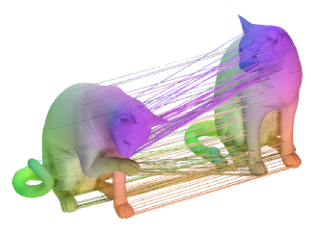
\includegraphics[height=5cm]{Pictures/cat.png}
\caption*{Source: [1]}
\end{figure}
\begin{enumerate}
\item[-] Assign each point from one point cloud to another point cloud such that the point and its image correspond to each other
\item[-] Could also use mesh information (faces) for computation
\end{enumerate}
\end{frame}

\section{Shape Correspondence via Divergence-Free Deformation Field}
\begin{frame}{What is a Divergence-Free Deformation Field?}
\begin{enumerate}
\item[-]Given two point clouds $X=\{x_1,...,x_n\} \subset \Omega, Y=\{y_1,...,y_n\}\subset \Omega$, find a mapping $f: \Omega \rightarrow \Omega$ s.t. $f(X)$ fits the shape $Y$
\item[-]Idea: $f$ should imitate real-world transformation from $X$ to $Y$
\item[-] What is natural? Smoothness and continuity!
\pause
\item[$\Rightarrow$]  \begin{equation*}
  	\begin{cases}
    \dot{x}(t) = v(x(t)) \\
    x(0) = x_n \\
    \end{cases}
    \end{equation*}
\item[-] $v: \Omega \rightarrow \mathbb{R}^D$ is called deformation field!
\begin{figure}
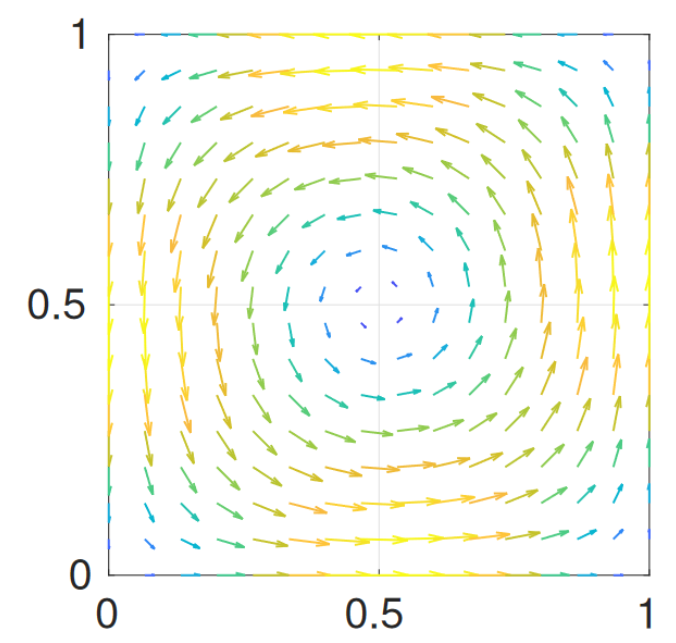
\includegraphics[height=3cm]{Pictures/deformation.png}
\caption*{Source: [2]}
\end{figure}
\end{enumerate}
\end{frame}
\begin{frame}{What is a Divergence-Free Deformation Field?}
\begin{enumerate}
\item[-]Two assumptions:
\begin{enumerate}
	\item Smoothness: $v \in C^\infty(\Omega, \mathbb{R}^D)$
	\item Divergence-free: $\triangledown\cdot v = 0 $
\end{enumerate}
\item[-]Why? Smoothness guarantees unique solution of IVP by Picard-Lindelöf
\pause
\item[-]Divergence-free vector fields conserve volume for any part $U \subset \Omega$ of the shape!
\begin{figure}
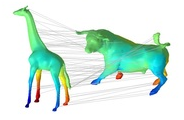
\includegraphics[height=3.5cm]{Pictures/badCorrespondence.png}
\caption*{Source: [3]}
\end{figure}
\end{enumerate}
\end{frame}

\begin{frame}{Obtaining the Correspondence Mapping}
\begin{enumerate}
\item[-] Evaluate solution operator at $t=1$ to get correspondence mapping $f$:\\ $f(x_n) := x(1)$
\item[-] t=1 is arbitrary and practical choice
\end{enumerate}
\end{frame}

\section{Representing the Deformation Field}
\begin{frame}{Representing the Deformation Field}
\begin{enumerate}
\item[-] We can now compute the correspondence given the deformation field
\item[-]But how to find the best deformation field? First, we need to represent the deformation field in an efficient way
\item[-] Compute a basis $\{v_1,v_2,...\}$ that spans the space of divergence-free deformation fields
\pause
\item[] \begin{equation*}
B_\phi = \left\{\phi: [0,1]^D \rightarrow\mathbb{R}, x \mapsto\prod_{d=1}^D \frac{1}{2}\sin(x_d\pi j_d) \big\vert j \in \mathbb{N}^D\right\}
\end{equation*}
\item[-] Sort the basis elements by eigenvalue
\pause
\item[-] Define $B_v = \bigcup_{k=1}^\infty\left\{\triangledown\times\begin{pmatrix}\phi_k\\0\\0\end{pmatrix}, \triangledown\times\begin{pmatrix}0\\\phi_k\\0\end{pmatrix}, \triangledown\times\begin{pmatrix}0\\0\\\phi_k\end{pmatrix}\right\}$
\item[$\Rightarrow$] $v(x) = \sum_{k=1}^K v_k(x)a_k$ for a fixed K.
\end{enumerate}
\end{frame}

\begin{frame}{Basis examples, sliced at $x_3=0.5$}
\begin{minipage}{.5\textwidth}
  \centering
  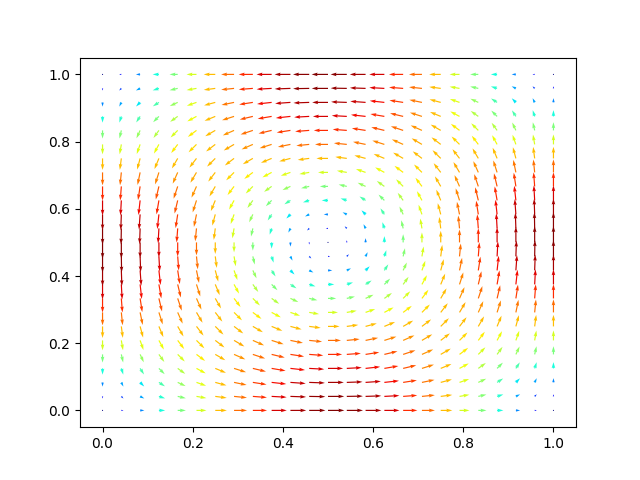
\includegraphics[height=4.3cm]{Pictures/basis1.png}
  \captionof*{figure}{$v_1$}
  \label{fig:test1}
\end{minipage}%
\begin{minipage}{.5\textwidth}
  \centering
  \includegraphics[height=4.3cm]{Pictures/basis2.png}
  \captionof*{figure}{$v_{12}$}
  \label{fig:test2}
\end{minipage}
\end{frame}

\section{Computing the Deformation Field}
\begin{frame}{Computing the Deformation Field}
\begin{enumerate}
\item[-] Remember: $v(x) = \sum_{k=1}^K v_k(x)a_k$
\item[-] We only have to find the correct $a_k$
\item[-] If we had the $a_k$ we could compute $f$ which maps $\{x_1,...,x_n\}$ to be in the shape of Y
\item[-] We still need to assign the points $f(x_n)$ to points $y_n$
\pause
\item[-] Idea: Do both at the same time with Expectation Maximization
\end{enumerate}
\begin{figure}
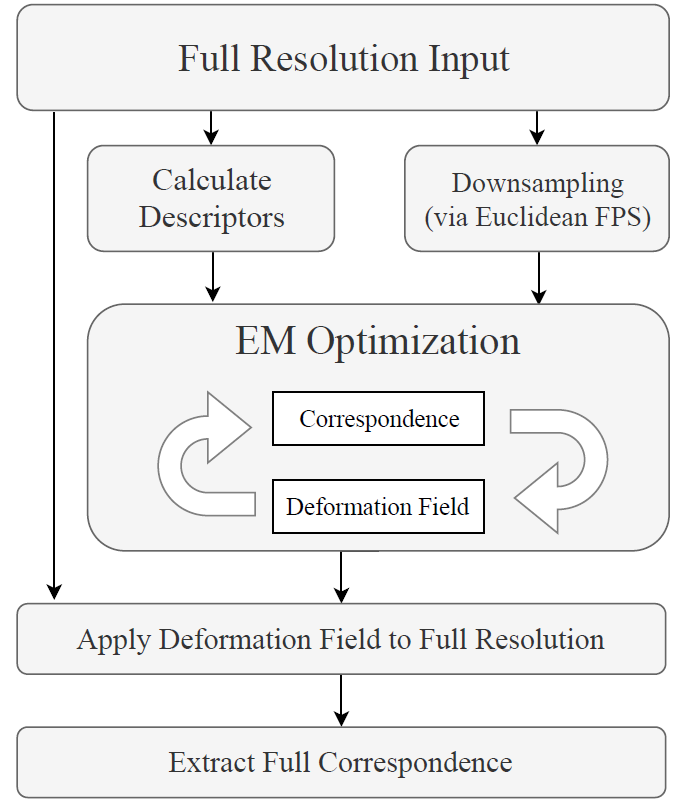
\includegraphics[height=4cm]{Pictures/Pipeline.png}
\caption*{Source: [2]}
\end{figure}
\end{frame}

\section{Shape Interpolation}
\begin{frame}{Shape Interpolation}
\begin{enumerate}
\item[-] Remember the IVP: \begin{equation*}
  	\begin{cases}
    \dot{x}(t) = v(x(t)) \\
    x(0) = x_n \\
    \end{cases}
    \end{equation*}
\item[-] We defined $f:=x(1)$
\item[-] What is $x(0.5)$?
\pause
\end{enumerate}
\begin{figure}
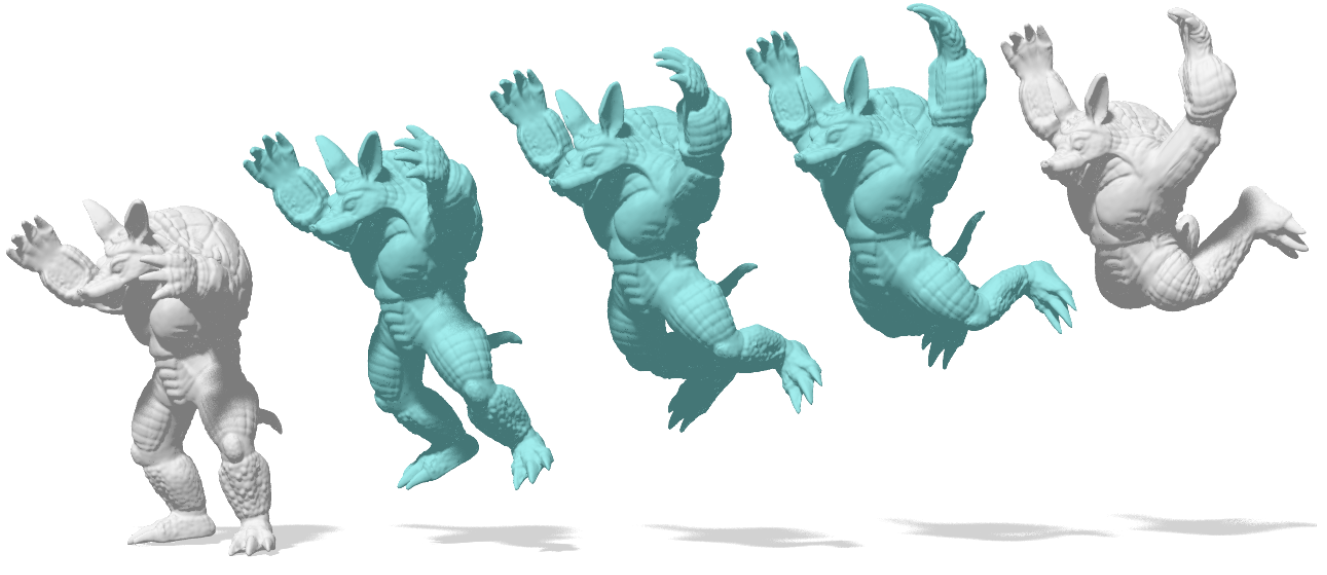
\includegraphics[height=4cm]{Pictures/Interpolation.png}
\caption*{Source: [2]}
\end{figure}
\end{frame}

\section{Project topic: Time-Varying Deformation Field}
\begin{frame}{Project topic: Time-Varying Deformation Field}
\begin{enumerate}
\item[-] There is only one time-independent deformation field
\end{enumerate}
\begin{figure}
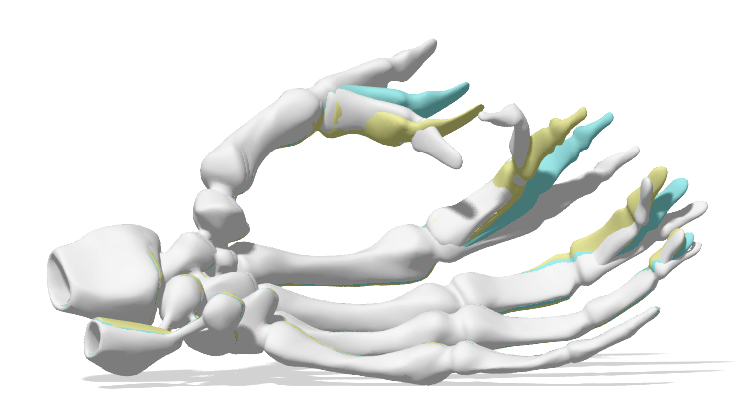
\includegraphics[height=4cm]{Pictures/hand.png}
\caption*{Source: [2]}
\end{figure}
\begin{enumerate}
\item[-] Possible Solution: Calculate multiple deformation fields for smaller timeframes
\item[-] Maybe even find a way to make deformation field vary over time
\end{enumerate}
\end{frame}

\section{Sources}
\begin{frame}{Sources}
\begin{enumerate}
\item[][1] \url{https://geoml.github.io/WI18/LectureSlides/L17_Functional_Map.pdf}
\item[][2] Eisenberger, Marvin, Zorah Lähner, and Daniel Cremers. "Divergence‐free shape correspondence by deformation." Computer Graphics Forum. Vol. 38. No. 5. 2019.1
\item[][3] \url{https://www.researchgate.net/figure/Shape-correspondence-results-Notice-that-our-method-is-not-confused-by-left-right-and_fig13_305750848}
\end{enumerate}
\end{frame}

%%%%%%%%%%%%%%%%%%%%%%%%%%%%%%%%%%%%%%%%%%%%%%%%%%%
\end{document}